% !TEX root = ../report.tex

\clearpage
\section{Elaborated model with patterns}
This section will describe the elaborated model on the basis of the patterns used in the architecture. For each patterns, this section will describe how it is implemented and how it affects the quality attributes of the system.

\subsection{Layers pattern}
\begin{figure}[H]
\centering
\includegraphics[scale=0.4]{7-software/images/Layers.png}
\caption{The Layers}
\label{fig:layers}
\end{figure}
The system is divided into four layers. The first layer is the presentation layer. This layer is responsible for handling the interaction with the end user. It contains the Web Interface, which is accessible to the user over HTTPS.

The second layer is the Service Layer, see Section~\ref{sec:service-layer-pattern} for more information about this layer. This layer offers services, which can be used by other (external) components.

The third layer is the Domain Layer and is responsible for the domain logic. The Domain Model contains all the classes, has an in-memory representation of the data and contains the logic which is inherent to the objects.
It uses the Unit of Work pattern (see Section~\ref{sec:unit-of-work-pattern}) to keep track of the changes to objects, so not every change will lead to a new database call. \\
The components in the Domain Layer are connected to the Domain Model, so they have access to the classes in there. \\
The Alerting component is responsible for sending alerts by email to the end user, for which it depends on an external Email Gateway. It also uses the StatisticsService in order to compute statistics, which it needs to decide if the user should be alerted by email. \\
The Configuration and Statistics components expose their functionality to the Service Layer.
% gateway is actually also a pattern :o

The Data Source layer contains the Unit of Work, which keeps track of the changes to the objects and translates those changes to database transactions when the object is committed. The layer also contains a Database Driver, which handles the communication with the database.

%TODO explain individual components (in one of the views?)


\subsection{Service Layer pattern}
\label{sec:service-layer-pattern}
The service layer encapsulates the application's business logic and defines the set of available operations/interfaces to clients. In Figure~\ref{fig:layers}, the Service Layer and its components can be seen. 

It contains the `StatisticsService', which exposes an interface used by clients to store the electricity usage data and is also used by the Web Interface for computing statistics. It is also used by the Alerts component in the Domain Layer, since it needs the same computed statistics as are displayed in the web interface, to decide if the user should be alerted by email.

The Service Layer also has the `Configuration Service', which is used by the Web Interface to allow the user to add new devices, change their properties or to configure new alerts.

The Service Layer makes a common set of application functionality available to many kinds of clients. This promotes the interoperability and also prevents having duplicate code.

\subsection{Unit of Work pattern}
\label{sec:unit-of-work-pattern}
\begin{figure}[H]
\centering
\includegraphics[scale=0.8]{7-software/images/UnitOfWork.png}
\caption{The Unit of Work class}
\label{fig:unitofworkclass}
\end{figure}

The Unit of Work pattern is used to keep track of the changes made to objects and newly created objects. Whenever an object is created, changed or deleted, the Unit of Work is told about this. 
Whenever the object can be saved to the database, the \verb|commit()| method of the Unit of Work is called, which translates the stored changes into database transactions.

A sequence diagram showing an example of this can be seen in Figure~\ref{fig:unitofworkseq}. Here, the StatisticsController constructs a new Device object, which is fetched from the database and then registers itself with the Unit of Work. When the StatisticsController changes the name of this device, the device object registers itself as dirty with the Unit of Work. 
When the device object is saved, it calls \verb|commit()| on the Unit of Work, which leads to the device updating the appropriate fields in the database.


\begin{figure}[H]
\centering
\includegraphics[scale=0.7]{7-software/images/UnitOfWorkSeq.png}
\caption{Sequence diagram showing an update to a Device-object using Unit of Work}
\label{fig:unitofworkseq}
\end{figure}

%It also uses an \textit{Identity Map} in order to guarantee that
  % explain this pattern somewhere


\clearpage
\subsection{Model-View-Controller}
\label{sec:mvc}
As mentioned in chapter \ref{ch:analysis}, MVC pattern is applied to decouple user-interface and the logic behind it. In this way, reusability is increased because the same models or controllers can be coupled with the same view. Modifiability is also increased because it becomes easier to modify a particular user interface or data model without interfering the logic, and vice-versa. Figure \ref{fig:mvc-architecture} depicts an example of MVC implementation in the HEMS.

\begin{figure}[H]
	\centering
	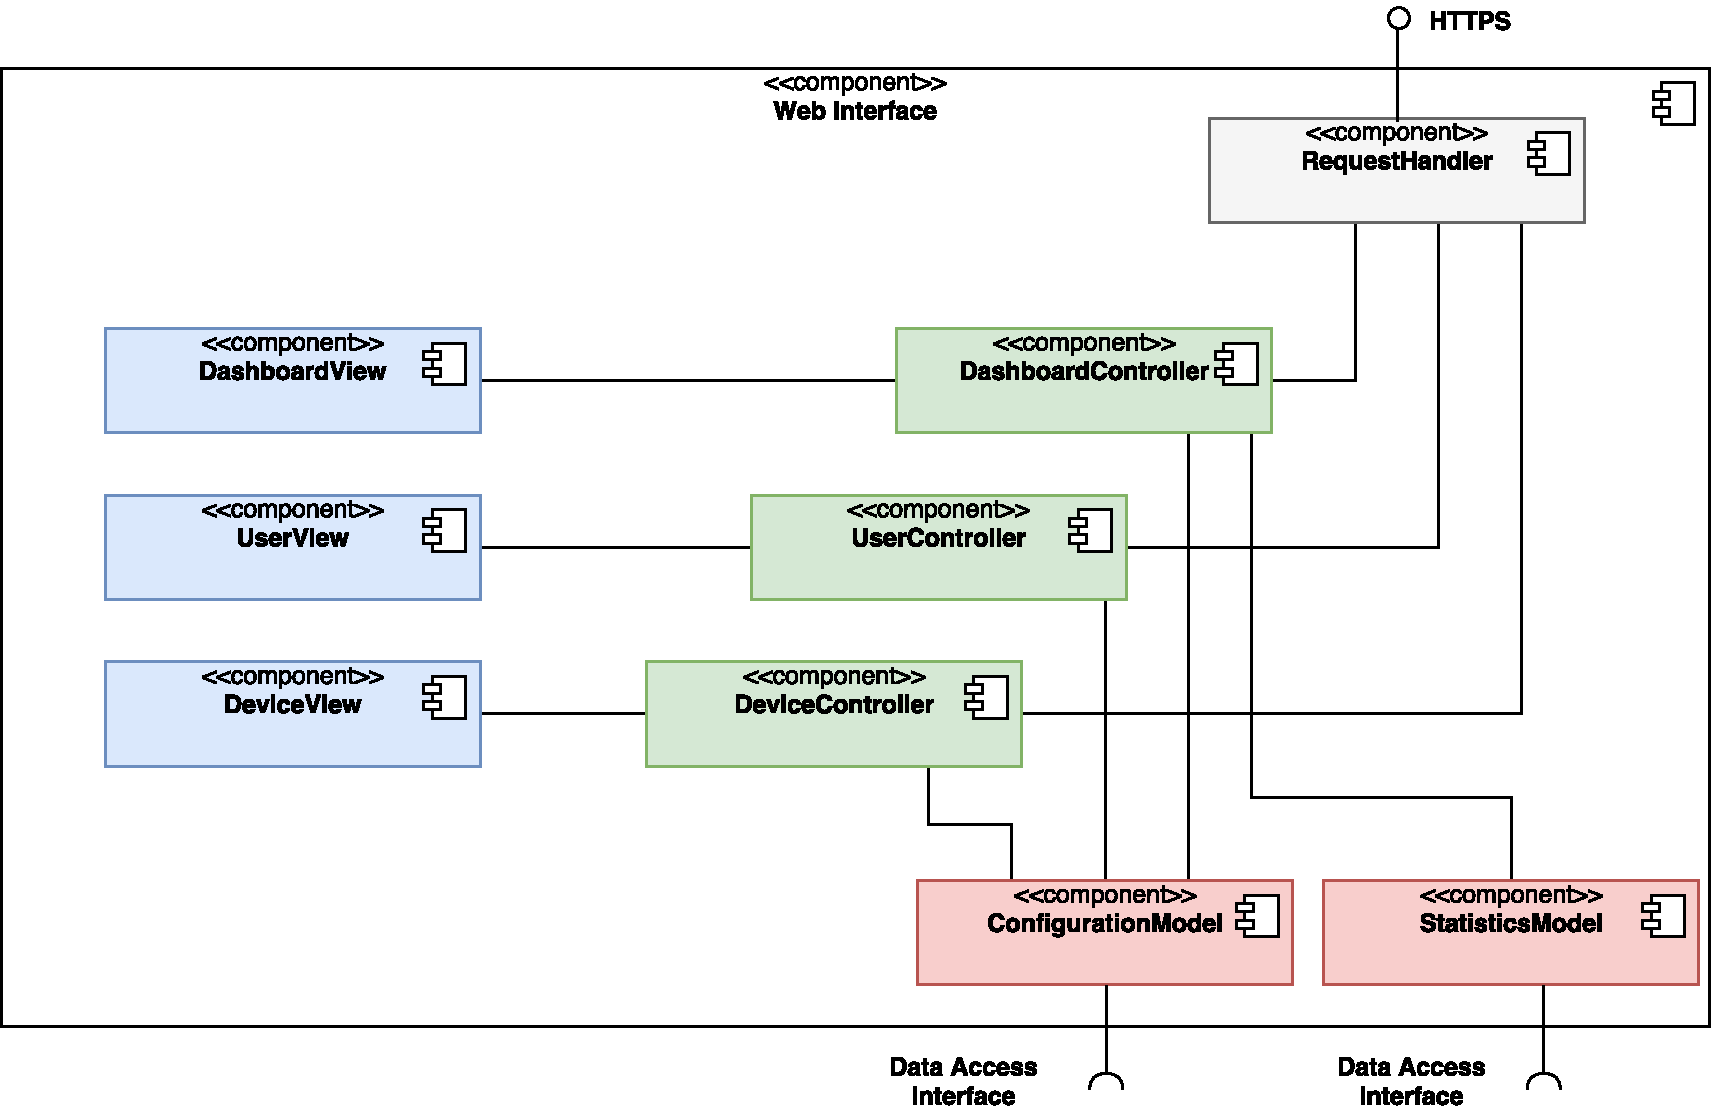
\includegraphics[width=0.8\textwidth]{7-software/images/mvc.pdf}
	\caption{Model-view-controller pattern implementation}
	\label{fig:mvc-architecture}
\end{figure}

Some models, views, and controllers are depicted in Figure \ref{fig:mvc-architecture}. Request handler handles incoming user request via HTTPS and routes it to the corresponding controller. Required data is then obtained through the models. Suitable views are used to provide user interface to the user. Some models, views, and controllers are presented in Figure \ref{fig:mvc-architecture}. However, there are more models, views, and controllers than those which are represented in the Figure \ref{fig:mvc-architecture}.

\clearpage
\subsection{Template View}
\label{sec:template-view}
Template view is implemented in this system to make the HTML code reusable in different pages. This will also make the view structure more simple. Code duplication can be prevented because instead of duplicating the code, the HTML will use a certain template.

\begin{figure}[H]
	\centering
	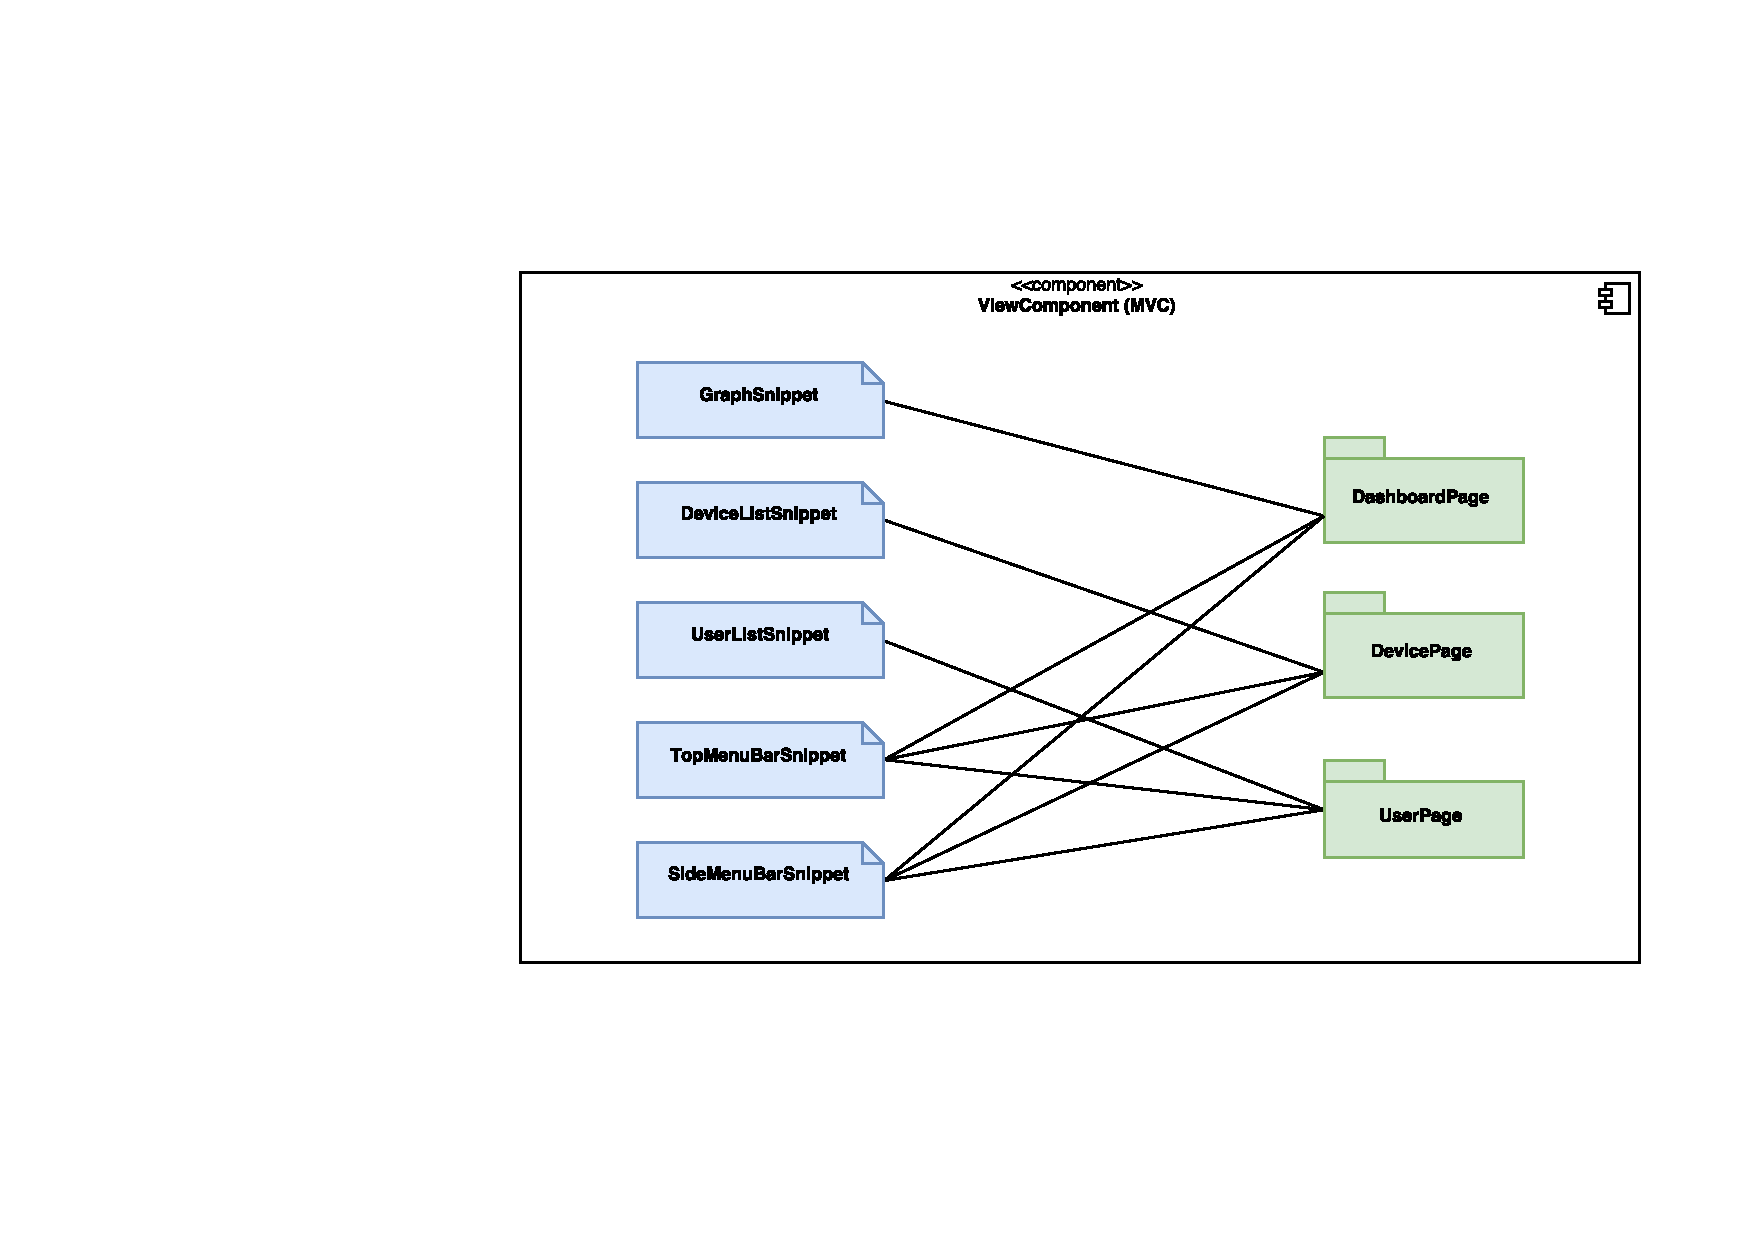
\includegraphics[width=0.7\textwidth]{7-software/images/template-view.pdf}
	\caption{Template view pattern implementation}
	\label{fig:template-view-architecture}
\end{figure}

Figure \ref{fig:template-view-architecture} shows an example of implementation of the template view pattern. Each page of the system (presented in green color) will combine several HTML code snippets (presented in blue color) together. \texttt{TopMenuBarSnippet} and \texttt{SideMenuBarSnippet} are used several times, as each page contains top menu bar and side menu bar. This is also good for expandability because the new page may just combine existing page template to create new web page.


